\section{Methodology}
\subsection{ARW-WRF Atmospheric Model and Large Eddy Simulation}
The WRF model is a state-of-the-art numerical mesoscale model that represent the latest scientific and engineering developments in climate prediction. It is open source, flexible, portable and efficient so that it allows simulations on both notebooks and massively parallelized supercomputers \citep{https://doi.org/10.5065/d68s4mvh}. In this work, the 3.8.1 version was used. It solves the non-hydrostatic Euler equations for fully compressible flow through a finite difference scheme. Spatial discretization is carried out through a C-Arakawa horizontal grid and a ground-following vertical grid based on hydrostatic dry air pressure. Temporal integration is carried out with a 2nd order Runge-Kutta scheme and the pressure waves that arises due to the model compressibility are filtered from the mean field through a divergence filter and are resolved in a time sub-step ($1/3$ of the external mode) to ensure the stability of the model. Boundary and initials conditions are specified from the results of a global model  A constant pressure condition with a damping layer is used at the upper boundary and wall functions are used at the soil surface through the surface layer parametrization.

%The high resolution is achieved by combining the dynamic downscaling of nested domains with the implementation of new databases for static information. The initialization of the internal domains is done through the downscaling of the results of the parent domains. In this way we will refer as mesoscale domains for those that meet $\Delta x > 1000$ (m) and microscale for $\Delta x < 500$ (m). 

The physical phenomena that lies within the model's mesh resolution are parameterized through several advanced schemes provided by the WRF team. Radiation, phase-change, cloud formation, surface interaction, boundary layer transport and turbulence are all considered within the model and are included in the right side of the equations as dependent terms. Regarding turbulence, for the mesoscale it is represented by a vertical eddy viscosity that is computed in the PBL parametrization subroutine, while the horizontal eddy viscosity is computed through a Smagorinsky closure \citep{smagorinsky1963general}. On the microscale, the PBL parametrization is turned off and a LES 1.5TKE  model is used \citep{deardorff1980stratocumulus}. The LES package in WRF \citep{Yamaguchi2012}, expresses the eddy viscosity as:
\be 
\nu_{t}=c_k \ell \sqrt{k},
\ee
where $c_k$ is the constant of the TKE model ($0.15\sim\! 0.30$) and $k$ is the sub-grid kinetic energy defined as:
\be 
k = \frac{1}{2}\tau_{nn}.
\ee 
The characteristic length $\ell$ of the model is computed as:
\begin{equation}
\ell = \begin{cases}\min[(\Delta x \Delta y \Delta z)^{1/3}, 0.76\sqrt{k}/N]&\quad N^2>0\\
(\Delta x \Delta y \Delta z)^{1/3}&\quad N^2\leq 0\end{cases}
\end{equation}
Where $N$ is the Brunt-Väisälä frequency for humid air. The value of $k$ in each domain cell is calculated based on the transport equation defined by  \cite{https://doi.org/10.5065/d68s4mvh}.

\subsection{Data Assimilation Process}
From the WRF model, three-dimensional arrays of  resolved meteorological variables (background) are obtained for a given time. The data assimilation (DA) goal is to physically weight the field measurements (observations) with these results to obtain the best estimate of the state of the atmosphere (analysis). Theoretically, the DA tries to minimize the cost function $J(x)$ that weighs the errors coming from the background $J_b$ and from observations $J_o$:
\be 
J(x)=J_b+J_o=\frac{1}{2}(x-x_b)^TB^{-1}(x-x_b)+\frac{1}{2}(Hx-y)^TR^{-1}(Hx-y)
\ee
Here $B$ is the background variance or error matrix (from the model), $R$ is the observation error matrix (from the instruments) and $H$ is the observation operator that performs a 3D interpolation of the numerical grid values to the observation space.  This equation is solved recursively using a Quasi-Newtonian minimization algorithm.
\begin{figure}[H]
	\centering
	\includegraphics[height=4cm,trim={5mm 3mm 3mm 3mm},clip,frame]{Imagenes/05/hov_dom1_edit.jpg}
	\includegraphics[height=4cm,trim={5mm 3mm 3mm 3mm},clip,frame]{Imagenes/05/hov_dom2_edit.jpg}
	\includegraphics[height=4cm,page=55,trim={43mm 87mm 20mm 4.5cm},clip]{Imagenes/06/hov/eta1_V}%
	\caption{(Left-Center) Simulation domains for H1-H2. (Right) Resolved velocity contour at the innermost domain at UTC 15:00. $\Delta x = 25$m in the innermost domain.}
	\label{fig:05_dom_hov}
\end{figure}
\subsection{Case Study Settings}
The goal of this study is to evaluate the behavior of the WRF mesoscale model in its LES mode when forced up to 3m mesh size while incorporating surface data assimilation within the PBL. 
Four experiments were developed for this purpose. The first two were carried out at Høvsøre \citep{Pea2015, Pea2013,floors2013wind} for the case without (H1) and with DA (H2). The last two correspond to simulations made in the Bolund Hill \citep{Berg2011,Bechmann2009,Bechmann2011} for the case without (B1) and with DA (B2). The simulation's high resolution is achieved through the implementation of non-native WRF databases and downscaling The ASTER database was used for the terrain height and Corine 2012 database \citep{Pineda2004} was used for land use category. As for the downscaling, nested domains with feedback were used (7 for H-experiments and 8 for B-experiment). The subdomains were selected as to avoid the double weighting due to the turbulent grey zone \citep{Wyngaard2004}. The standart 3:1 ratio was used in the meso and microscale and a 5:1 ratio \citep{Green2015} for the domains where the shift to the microscale occurs (\emph{terra incognita}). Initial and boundary condition of the coarser mesh is given by the operational analysis of the GFS global model with 0.5$^\circ$ of resolution. The boundary condition was mapped to the first domain border using a buffer zone of 5 elements of mesh and are updated every 6 hours. The configuration of the domains was subjected to a sensitivity analysis in order to adjust the best values to ensure: (i) the model stability, (ii) the convergence of results for the boundary layer and (iii) the lowest computation time. In this fashion, the number of elements for the mesh and the top boundary condition are established. The number of nodes in all the domains are set as $107\times107\times37$ for H-experiments and $107\times107\times41$ for B-experiment (except for the innermost domain which is $107\times92\times41$ due the terrain database). For the vertical mesh, special care is taken to refine it so it is consistent with the application of the LES. In the first level there is an aspect ratio of $\Delta_x/\Delta_{z_1}=2.35$ (see Figure \ref{fig:05_mesh_bol}) and this is progressively reduced in the higher levels. Lastly, the data needed to feed the data assimilation process comes from meteorological masts located within the innermost domain in each experiment. For the H-experiments there is one mast located at the center and for the B-experiments there are 8 masts distributed as shown in Figure \ref{fig:05_mesh_bol}. The frequency at which the background is corrected is set at 10 minutes and is performed during the first 6 hours of the simulation. The variables that were assimilated are wind speed and direction, and are assimilated at 10, 40, 60, 80 and 100 meters above the ground for H-experiments and 2,5 and 9 meters for B-experiments.

For H-experiments, the performed simulations consists of a total of 14 hours, where the first 6 correspond to the spinup of the model and the time window where the data assimilation is applied. The date of the simulation were selected in such a way that it corresponds to a period with neutral atmospheric stability as declared by \cite{Pea2013} in its case 5, i.e. 08/09/2010 from 06:00 to 20:00, and the validation was done through comparison with values from that measurement campaign.
\begin{figure}[H]
	\centering
	\includegraphics[height=4cm,trim={0cm 5mm 0cm 0cm},clip]{Imagenes/05/hd_mesh_50}%
	\includegraphics[height=4cm,page=1,trim={3.4cm 9.3cm 1cm 4cm},clip]{Imagenes/05/bol_control_point.pdf}%
	\includegraphics[height=4cm,page=109,trim={37mm 30mm 45mm 22mm},clip]{Imagenes/06/bol/eta1}%
	\caption{(Left) Detail the steep slope in M1-M4 cut. (Center) Control points locations for B1-2. (Right)  Resolved streamlines in the first level of B1 at UTC 15:00.$\Delta x = 2,74$m in the innermost domain.}
	\label{fig:05_mesh_bol}
\end{figure}
%Bolund is a 12 [m] high, 130 [m] long and 75 [m] wide seaside hill located in Denmark. Thanks to the measurement campaign made by \cite{Bechmann2009}  and its posterior blind model comparison \citep{Berg2011,Bechmann2009,Bechmann2011}, this is an optimal location for the testing of experimental computational models who attempt to simulate complex terrain. The measurement campaign provides Bolund with information on 10 masts distributed across and close to the hill, as well as high resolution data for terrain height and roughness length.

The B-experiments consisted of 9 hours of simulation, with the first 6 hours being used for spinup and DA. The date was selected according to what was declared by  \cite{Bechmann2009} for a day with the most neutral stratification possible, i.e. 29/12/2007 from 06:00 to 15:00. The validation was carried out by contrasting the values given for the blind comparison.

To evaluate the performance of the simulations in relation to the real data, RMSE and the MAE applied to the wind speed are used as metrics.
\begin{align}
MAE = \frac{1}{n}\sum_{i=1}^n|V_m-V_o|\quad;\quad
RMSE= \sqrt{\frac{1}{n}\sum_{i=1}^n(V_m-V_o)^2}
\end{align}
Where $V_o$ is the observed speed and $V_m$ is the modelled speed. The evaluation these metrics was performed after the spinup time and each of the measured values is compared with the nearest simulated value, interpolated to the corresponding height in the mast. The interpolation is made using a simple logarithmic law for the wind profile,
\be 
u(z)=u(z_r)\frac{\ln(z/z_0)}{\ln(z_r/z_0)}
\ee
Where $z_0$ is the corresponding roughness length for each case \citep{Pea2013,Bechmann2011}.








